\section{ЧАСТЬ 2}

\subsection{Задание}

Написать загружаемый модуль ядра, создать файл в файловой
системе {\ttfamily proc}, {\ttfamily sysmlink},
{\ttfamily subdir}. Используя соответствующие
функции передать данные из пространства пользователя в
пространство ядра (введенные данные вывести в файл ядра)
и из пространства ядра в пространство пользователя.

\subsection{Листинги}

\begin{lstlisting}[caption=Код модуля]
#include <linux/module.h>
#include <linux/moduleparam.h>
#include <linux/init.h>
#include <linux/kernel.h>
#include <linux/proc_fs.h>
#include <asm/uaccess.h>
#include <linux/vmalloc.h>

#define MAX_COOKIE_LENGTH PAGE_SIZE

MODULE_LICENSE("Dual BSD/GPL");
MODULE_AUTHOR("Alexander Stepanov");

static struct proc_dir_entry *proc_entry;
static struct proc_dir_entry *proc_directory;
static struct proc_dir_entry *proc_link;
static char *cookie_pot;
static int cookie_index;
static int next_fortune;

static ssize_t fortune_write(struct file *f, const char __user *buff,
    size_t len, loff_t *data)
{
    int space_available = (MAX_COOKIE_LENGTH - cookie_index) + 1;

    if (len > space_available)
    {
        printk(KERN_INFO "fortune: cookie pot is full!\n");
        return -ENOSPC;
    }

    if (copy_from_user(&cookie_pot[cookie_index], buff, len))
    {
        return -EFAULT;
    }

    cookie_index += len;
    cookie_pot[cookie_index-1] = 0;

    return len;
}

static ssize_t fortune_read(struct file *f, char __user *buff,
    size_t len, loff_t *data)
{
    if (*data > 0) return 0;

    if (next_fortune >= cookie_index)
        next_fortune = 0;

    len = copy_to_user(buff, &cookie_pot[next_fortune], len);
    next_fortune += len;

    *data = 1;

    return len;
}

static struct file_operations ops =
{
    .owner = THIS_MODULE,
    .read = fortune_read,
    .write = fortune_write,
};

static int md_init(void)
{
    int ret = 0;
    cookie_pot = (char *)vmalloc( MAX_COOKIE_LENGTH);

    if (!cookie_pot)
    {
        ret = -ENOMEM;
    }
    else
    {
        memset(cookie_pot, 0, MAX_COOKIE_LENGTH );
        proc_entry = proc_create("fortune", 0644, NULL, &ops);

        if (proc_entry == NULL)
        {
            ret = -ENOMEM;
            vfree(cookie_pot);
            printk(KERN_INFO "fortune: Couldn't create proc entry\n");
        }
        else
        {
            cookie_index = 0;
            next_fortune = 0;
            printk(KERN_INFO "fortune: Module loaded.\n");

            proc_directory = proc_mkdir("fortune_dir", NULL);

            if (proc_directory == NULL)
            {
                ret = -ENOMEM;
                printk(KERN_ERR "fortune: Couldn't create dir");
            }

            proc_link = proc_symlink("fortune_link", NULL, "fortune");

            if (proc_link == NULL)
            {
                ret = -ENOMEM;
                printk(KERN_ERR "fortune: Couldn't create symlink");
            }
        }
    }

    return ret;
}

static void md_exit(void)
{
    proc_remove(proc_entry);
    proc_remove(proc_directory);
    proc_remove(proc_link);
    vfree(cookie_pot);
    printk(KERN_INFO "fortune: Module unloaded.\n");
}

module_init(md_init);
module_exit(md_exit);
\end{lstlisting}

\subsection{Результат работы}

\begin{figure}[H]
    \centering
    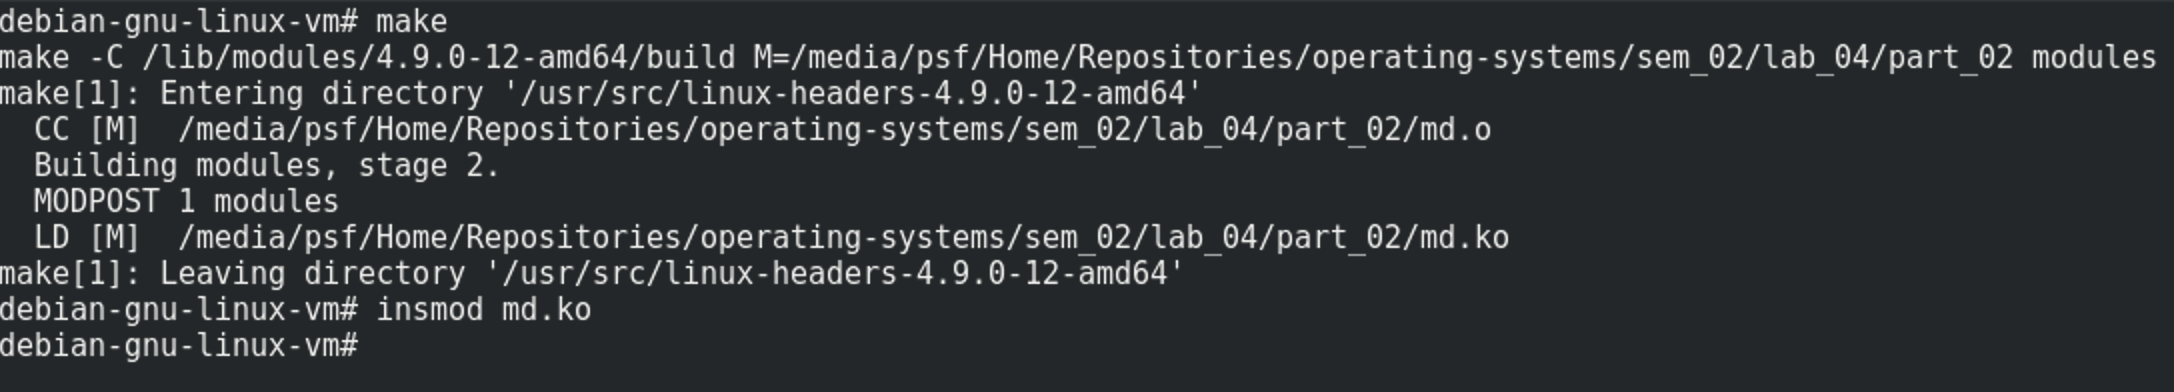
\includegraphics[scale=0.45]{img/part_02/make.png}
    \caption{Сборка и загрузка модуля}
\end{figure}

\begin{figure}[H]
    \centering
    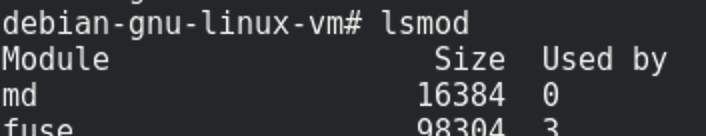
\includegraphics{img/part_02/lsmod.png}
    \caption{Модуль загружен}
\end{figure}

\begin{figure}[H]
    \centering
    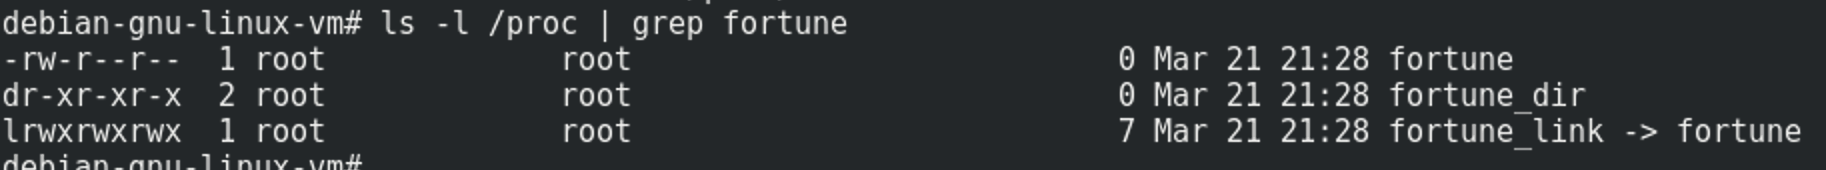
\includegraphics[scale=0.55]{img/part_02/ls.png}
    \caption{Модуль создал файл, символьную ссылку и директорию}
\end{figure}

\begin{figure}[H]
    \centering
    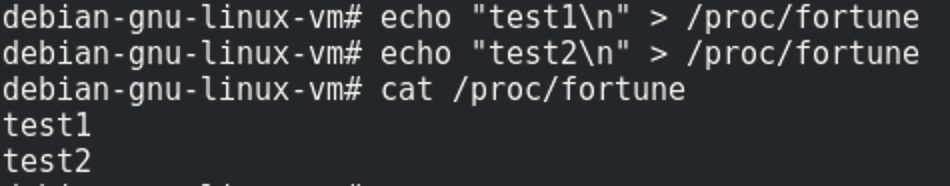
\includegraphics{img/part_02/test_file.png}
    \caption{Проверка работы файла}
\end{figure}

\begin{figure}[H]
    \centering
    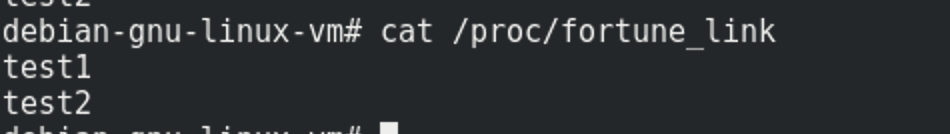
\includegraphics{img/part_02/test_link.png}
    \caption{Проверка работы ссылки}
\end{figure}

\subsection{Обоснование использования специальных функций}

В linux память сегментирована, это значит, что указатель не
ссылается на уникальную позицию в памяти, а ссылается на
позицию в сегменте. Процессу доступен только собственный сегмент
памяти. Если выполняется обычная программа, то адресация
происходит автоматически. Если выполняется код ядра и необходимо
получить доступ к сегменту кода ядра, то всегда нужен буфер, но
когда мы хотим передать информацию между процессом и кодом ядра,
то соответствующая функция ядра получит указатель на буфер процесса.
